\section{Experiments and results}\label{chapter4}

\subsection{Dataset}

%Just say how many samples and how many features, why 'multiple'?
%We also observed that the original training dataset might be applied with PCA and reduced the dimension to $60000 \times 128$ matrix.
%The training label is a $60000 \times 1$ matrix.
%Similarly, the testing dataset is $10000 \times 128$ matrix.
This is a result section, just states your result. Describe the dataset.

Our neural network is designed to classify $10,000$ unlabelled samples with $128$ features and $10$ different classes, using $60,000$ similar labelled samples. As described in Section~\ref{sec:early}, we split the labelled dataset into $50,000$ training samples and $10,000$ cross validation samples. The features in the dataset ranges from $-2045.92$ to $2803.84$, as illustrate in Figure~\ref{put a frequency plot here.}.



%Then we use all the $60,000$ samples to build our final neural network model.


\subsection{Multiprocessing speed up hyperparameters tuning}
%We apply three layers neural network model with three different activation functions such as tanh, sigmoid and ReLu for the hidden layers as well as a Softmax activation function for the output layer.
%We apply batch normalisation to the input for each layer to reduce the training time and make our model more resilient to parameter scale.
%As for the regularisation techniques,
%we use early stopping, drop out and weight decay to prevent over-fitting.
%We use combinations of all the above setups to tune the hyperparameters for our neural network model,
%in the end we successfully find the benchmark model to use for prediction with best accuracy and reasonable runtime.
We use \texttt{python} 3.6 to code the neural network model with a list of library dependencies specified in the file named \texttt{requirements.txt} file in our git repository. In particular, \texttt{scipy} 1.21 ....

We write a shell script to run all our tests in parallel in a high performance computer, whose hardware specification is shown in Figure~\ref{fig:hardware}. The shell script trains our model with various hyperparameters from different 
\texttt{json} files in parallel. 
Running multiple experiments in parallel allows us to fully utilise our computing resources, and tune hyperparameters efficiently. Although the speed for each task has been dropped by $30\%$, this parallel setting dramatically reduces the total running time required to finish the nine experiments detailed in Tables~\ref{table:best-four-steps} and~\ref{tb:comp}. For example, fitting our neural networks with these nine different sets of hyperparameters in parallel takes $17.2$ minutes, which is the time required by run~3 (Table~\ref{table:best-four-steps}). However, fitting the nine neural networks in sequence takes a total of $38$ minutes, which doubles the total time required in the parallel setting. 

%\begin{lstlisting}[language=bash,caption={bash version}]
%#!/bin/bash

%python3 Neural_Network.py --config=./config/8987.json &
%python3 Neural_Network.py --config=./config/batch_size_60000.json &
%python3 Neural_Network.py --config=./config/no_weigh_decay.json &
%python3 Neural_Network.py --config=./config/no_momentum.json &
%python3 Neural_Network.py --config=./config/dropout_05.json &

%python3 Neural_Network.py --config=./config/8987.json &
%python3 Neural_Network.py --config=./config/8995.json &
%python3 Neural_Network.py --config=./config/8972.json &
%python3 Neural_Network.py --config=./config/8975.json &
%python3 Neural_Network.py --config=./config/8932.json &
%\end{lstlisting}

\begin{figure}
    \center{
        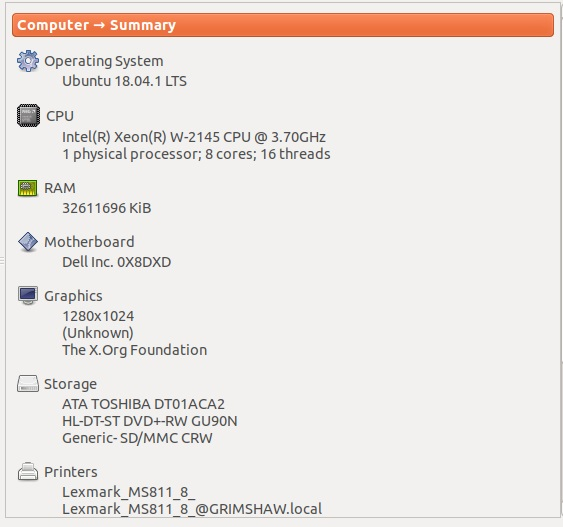
\includegraphics[scale=0.8]{resource/hardware.png}
    }
    \caption{Hardware to run the tests.}
    \label{fig:hardware}
\end{figure}




\subsection{Experiments Results}
\subsubsection{Early stopping decides maximum number of iterations}
%Early stopping is a form of regularisation technique we use to avoid over-fitting for our neutral network,
%it guides us on how many iterations can be run before the model begins to over-fit.
As discussed in Section~\ref{sec:early}, we split given labelled dataset into $50,000$ training samples and $10,000$ cross validation samples. Cross validation finds $44$ iterations gives the best cross validation accuracy, which is 89.6\% (Figure~\ref{fig:acc-iter}). As a result, we choose $44$ iterations as our early stopping point for the benchmark model. 

% shows that the cross validation accuracy of our benchmark model reaches a maximum (89.6\%) has at the $44$th iteration. After then, ...

\begin{figure}
	\centering{
	%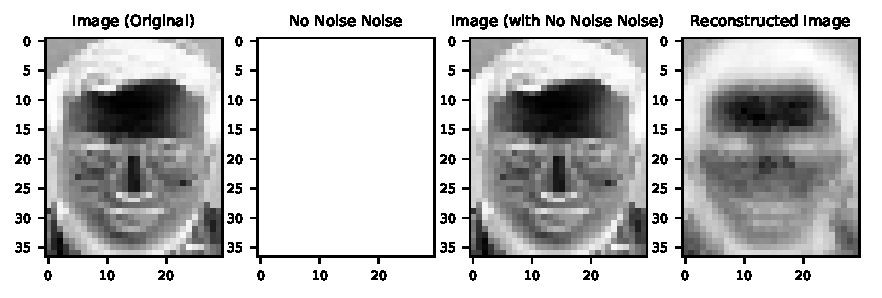
\includegraphics[scale=.9]{Result_Multiplication_KL_Divergence_No_Noise_Comparison}
	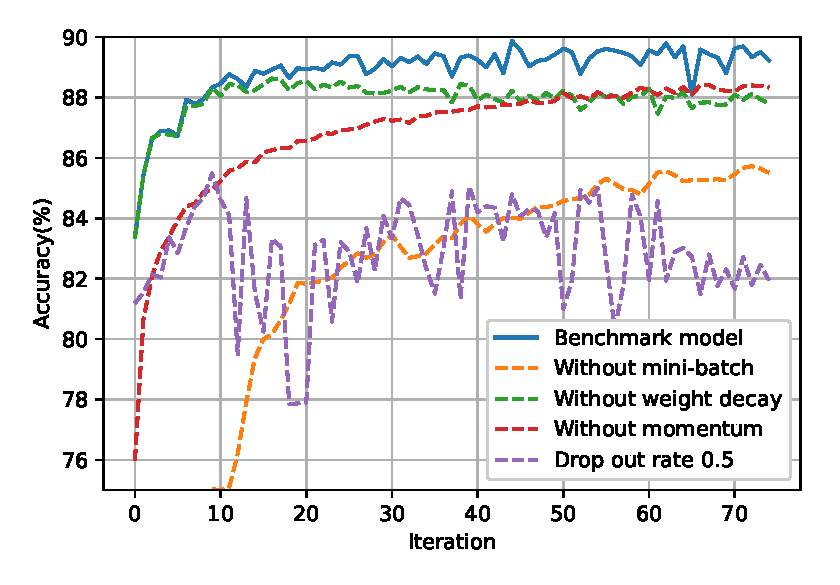
\includegraphics
    {resource/acc2.eps}}
    \caption{Results and parameters of different setups for 89.87}
    \label{fig:acc-iter}
\end{figure}

\subsubsection{Optimal hyperparameters}
Table~\ref{table:best-four-steps} shows cross validation accuracy and hyperparameters with optimal and sub-optimal coefficients. The benchmark model achieved the accuracy of $89.9\%$.
% After 44 iter, the cross validation is almost same, but training acc still going up - overfit
% No weight decay - going down
% no momentum - slow
% Dropout rate 
% without mini batch - slow

\begin{table}
\caption{Hyperparameters for models with outstanding cv accuracy.\label{table:best-four-steps}}
\centering
{\footnotesize
\begin{tabular}{@{}lrrrrr@{}}
\toprule
Experiment                & Benchmark  & Test 2           & Test 3           & Test 4  & Test 5  \\ \midrule
Run time (minutes)             & 2.3     & 2.7              & 3.6              & 17.2    & 10.8    \\
CV Accurarcy                 & 89.9\%  & 89.7\%           & 89.8\%           & 90.0\%  & 89.3\%  \\
Initialisation            & Xavier  & \parbox[T]{1cm}{Uniform$(-1,1)$} 
& \parbox[T]{1cm}{Uniform$(-1,1)$} 
                                                                            & Xavier  & Xavier  \\
Batch size                & 1500    & 1500             & 1500             & 1500    & 1500    \\
Hidden layer nodes        & 160     & 150              & 150              & 900     & 160     \\
Activation function       & $\tanh$ & $\tanh$          & $\tanh$          & $\tanh$ & sigmoid \\
Weight decay rate         & 0.0007  & 0.0007           & 0.0007           & 0.007   & 0.007   \\
Momentum rate             & 0.9     & 0.9              & 0.92             & 0.9     & 0.9     \\
Dropout rate              & 0.95    & 1.0              & 1.0              & 0.5     & 0.95    \\
Learning rate             & 0.11    & 0.05             & 0.05             & 0.11    & 0.11    \\
Optimal iteration & 44      & 54               & 66               & 158     & 282     \\ 
BN & True      & True          & True          & True       & True          \\\bottomrule
\end{tabular}
}
\end{table}


\begin{table}
\caption{Accuracies and parameters of different setups for 89.87 results. Rows are columns are.\label{tb:comp}}
{\footnotesize \centering
\begin{tabular}{@{}lrrrrrr@{}}
\toprule
Experiment                  & Drop out 50\% & Momentum & Weight decay & Mini-Batch & BN \\ \midrule
Run time (minutes)             & 0.5        & 8.6          & 0.8      & 7.6 & 4.5          \\
CV Accurarcy                   & 85.5\%     & 89.4\%       & 88.6\%   & 87.5\% &82.8\%       \\
Initialisation              & Xavier     & Xavier       & Xavier   & Xavier & Xavier        \\
Batch size                   & 1500       & 1500         & 1500     & 60000    & 1500        \\
Hidden layer nodes        & 160        & 160          & 160      & 160    & 160         \\
Activation function        & $\tanh$    & $\tanh$      & $\tanh$  & $\tanh$  & $\tanh$       \\
Weight decay rate          & 0.0007     & 0.0007       & 0        & 0.007  & 0.007        \\
Momentum rate                & 0.9        & 0            & 0.9      & 0.9    & 0.9         \\
Dropout rate                & 0.5        & 0.95         & 0.95     & 0.95    & 0.95        \\
Learning rate                & 0.11       & 0.11         & 0.11     & 0.11    & 0.11       \\
Optimal iteration       & 9          & 198          & 16       & 177     & 80       \\ 
BN       & True          & True          & True       & True     & False       \\ \bottomrule
\end{tabular}
}
\end{table}

% \begin{figure}
%     \center{\includegraphics
%     {resource/acc.eps}}
%     \caption{\label{fig:my-label2}Results and parameters of different setups for 89.87 results.}
% \end{figure}

\begin{figure}
    \center{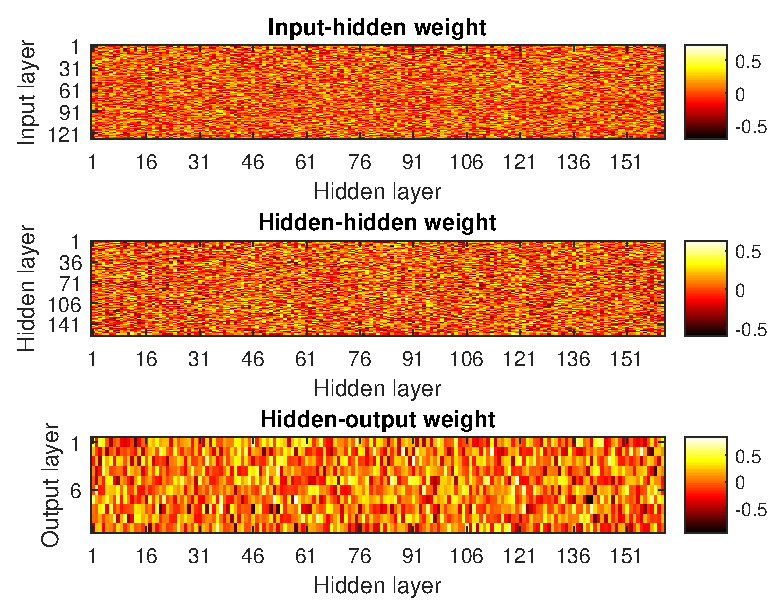
\includegraphics
    {resource/figure2.eps}}
    \caption{\label{fig:my-label3}Weight Matrices for our benchmark model.}
\end{figure}


\subsection{Experiments Results}

\subsubsection{Vectorisation dramatically improves the speed of training}
%We used vectorisation from numpy to perform fast computation and transformation of the data rather than using the traditional for-loop,
%these operations includes matrix concatenation, multiplication, divide using Numpy libraries.
This is a result section, you only need to state result, i.e. run the model with batch size =1 and compare the speed etc and ONLY state your results. If you want to say something about the method please put it into the method section.

\subsubsection{BN significantly improves the accuracy}


\subsubsection{Weight decaying prevents over-fitting}


\subsubsection{dropout helps for large neural networks}

You need to report the parameter for bench mark models.
How other models compare with bench mark models.